
\documentclass{llncs}

\usepackage{llncsdoc}

\usepackage{times}            % standard fixed width font
\usepackage{graphicx}
\usepackage{amsmath}
\usepackage{xspace}
\usepackage{footnote}
\usepackage{cite}
\usepackage{subfig}
%\usepackage{natbib}

%\usepackage{multirow}
\usepackage{setspace} 
\usepackage{epsfig}
\usepackage[hyphens]{url}
\usepackage[colorlinks,linkcolor=blue,citecolor=blue,urlcolor=blue]{hyperref}
\usepackage[hyphenbreaks]{breakurl}
\usepackage{booktabs}
%\usepackage[compact]{titlesec}
\usepackage{xcolor}
%\usepackage[algoruled,vlined,ruled,linesnumbered]{algorithm2e}
\usepackage{lipsum}
\usepackage{courier}
\usepackage{listings}
\lstset{
  language=C,
	basicstyle=\footnotesize\ttfamily,breaklines=true
}

%\usepackage[T1]{fontenc}
%\usepackage[scaled=0.78]{DejaVuSansMono}

\clubpenalty=10000      % penalty for creating a club line at end of line.
\widowpenalty=10000     % penalty for creating a widow line at top of page.

% Select one or other if want to see comments.
% \com is sometimes displayed during draft.
\long\def\com#1{}
%\long\def\com#1{{\bf \sc comment: }{\small [#1]}{\bf \sc\ endcomment}\newline}

\long\def\xxx#1{{\color{red}{\bf XXX: }{\small [#1]}}}
\long\def\ruzica#1{{\color{red}{\bf Ruzica: }{\small [#1]}}}
%\long\def\xxx#1{}

% Use this macro to force page breaks where ugly widows/orphans occur;
% be sure to recheck all uses after any significant change to the text!
\def\widowpage{\pagebreak}

% Choose abbreviated or long-version alternatives in paper
%\long\def\abbr#1#2{#1}			% abbreviated version
\long\def\abbr#1#2{#2}			% long version

% Choose abbreviations or long names/titles in bibliography
%\def\bibbrev#1#2{#1}			% short version
%\def\bibbrev#1#2{#2}			% long version
\def\bibbrev#1#2{\abbr{#1}{#2}}		% follow abbr macro

% Abbreviated or full citation lists: \abcite{basic}{others}
\newcommand{\abcite}[2]{\abbr{\cite{#1}}{\cite{#1,#2}}}

% Conference abbreviations: \bibconf[Nth]{SOSP}{Symposium on ...}
\newcommand{\bibconf}[3][]{#1 \bibbrev{#2}{#3 (#2)}}

\newcommand{\ie}{{\em i.e.\xspace}}
\newcommand{\eg}{{\em e.g.\xspace}}

% system related terms
\newcommand{\app}{ConfigC\xspace}

% Fault graph terms

\newcommand{\para}[1]{\smallskip\noindent {\bf #1}}

\begin{document}

\special{papersize=8.5in,11in}
\setlength{\pdfpageheight}{\paperheight}
\setlength{\pdfpagewidth}{\paperwidth}

% Uncomment one of the following two, if you are not going for the 
% traditional copyright transfer agreement.

%\exclusivelicense                % ACM gets exclusive license to publish, 
                                  % you retain copyright

%\permissiontopublish             % ACM gets nonexclusive license to publish
                                  % (paid open-access papers, 
                                  % short abstracts)

%\titlebanner{banner above paper title}        % These are ignored unless
%\preprintfooter{short description of paper}   % 'preprint' option specified.

\title{Probabilistic Automated Language Learning for Configuration Files}

\author{~}
\institute{~}
\maketitle


\section*{Abstract}

System failures resulting from configuration errors 
are major reasons for compromised availability and
reliability of today's software systems.
Although many misconfiguration handling techniques
such as checking, troubleshooting, and repair
have been proposed, 
offering automatic verification for configuration files -- as often  
done for regular programs -- is still an open problem.
This is because software configurations are typically written in
poorly structured and untyped ``languages'', and 
specifying constraints and rules for configuration 
verification is non-trivial in practice.

This paper presents \app, the first automatic verification framework for
general software configurations.
\app verifies a target configuration file $F$ through three steps.
Firstly, \app analyzes a dataset containing many sample configuration 
files belonging to the same system as $F$,
translating these sample files to a
well-structured and probabilistically-typed 
intermediate representation.
Secondly, \app derives rules and constraints by analyzing
this intermediate representation, thus building a
sophisticated language model.
Finally, \app uses the resulting language model to verify $F$.
The \app framework is highly modular, 
does not rely on system source code, and
can be applied to any new configuration file type with minimal user input. 

\app is capable of detecting various errors that cannot
be detected by previous efforts,
including entry ordering errors, fine-grained value correlation errors, 
and missing entry errors. 
We evaluate \app using a real-world dataset with 261 incorrect 
MySQL configuration files,
and \app is able to correctly 
detect errors (previous work failed to
detect) in 217 files.

%\section*{Outline}

\begin{itemize}

\item Introduction: 

\item Motivating examples: Put two or three misconfiguration
  examples here, and show why they are incorrect.

\item \app Design: 
  \begin{itemize}
  \item Present an architecture of \app with a fig. Briefly describe 
    how it works (step by step).
  \item Detail learner part
  \item Merge
  \item Check 
  \item Limitations
  \end{itemize}

\item Implementation and Evaluation:
  First, briefly describe how we implemented \app.
  Then, show a few results, \eg, benchmark including learning time,
  checking time (with different size of configuration file).
  Case study?  I am not sure.

\end{itemize}





\section{Introduction and System Overview}
\label{sec:Intro}

Configuration errors are one of the most important root-causes of
modern software system failures~\cite{xu15systems,yin11anempirical}.
In practice, misconfiguration problems may result in security
vulnerabilities, application crashes, severe disruptions in software
functionality, and incorrect program executions%
~\cite{xu15systems,zhang14encore,yuan11context}.  Although several
tools have been proposed to automate configuration error diagnosis
after failures occur~\cite{wang04automatic,attariyan10automating,
su07autobash,whitaker04configuration}, these tools rely on a manual approach
  to understand and detect the failure symptoms. The main reasons for this are:
  1) entries in configuration files are untyped assignments, 2) there
  is no explicit structure policy for the entries in configuration
  files, and 3) there are surprisingly few rules specifying the
  entries' constraints.

We propose an approach to the verification of  
configuration files which is based on learning rules about the language 
model for configuration files. 

\begin{figure}[t] \centering
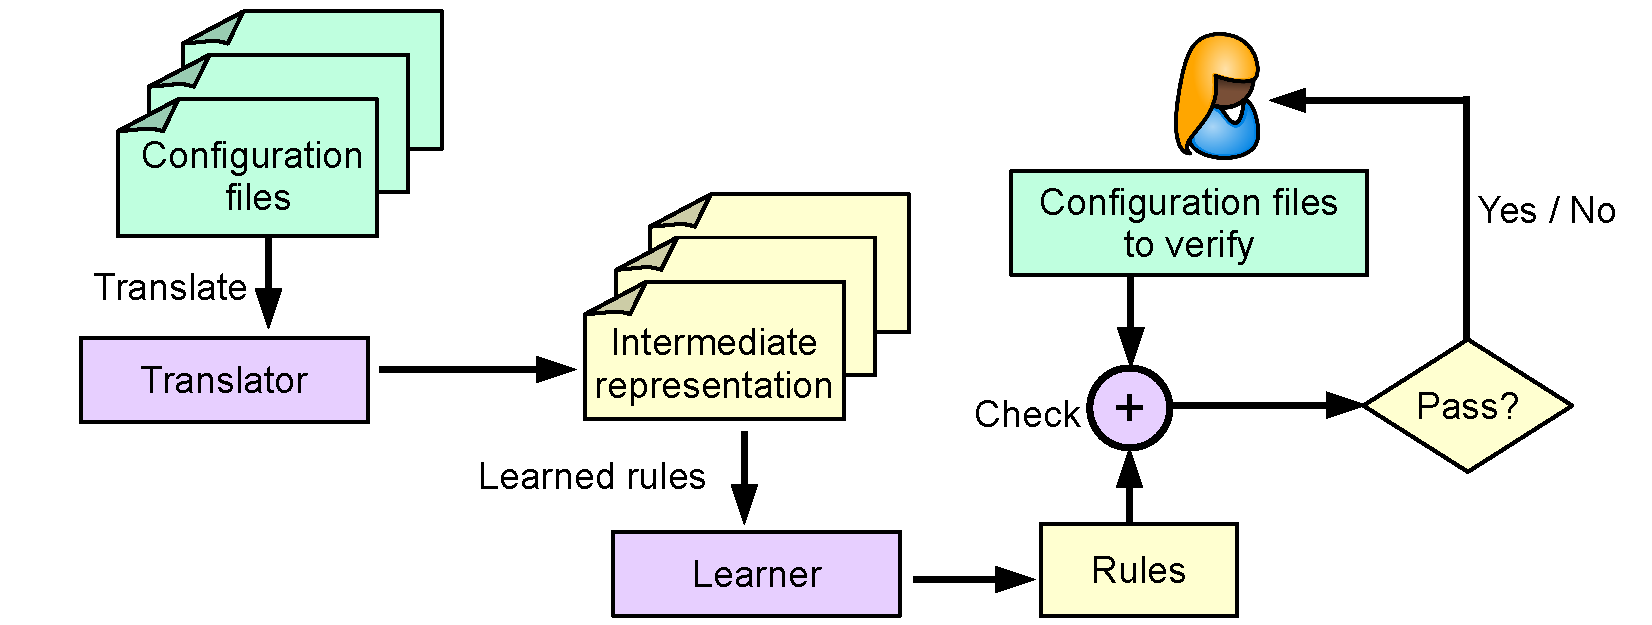
\includegraphics[width=0.65\textwidth]{figs/overview}
\caption{{\footnotesize \app's workflow. The green boxes represent configuration files,
  including both correct general configuration files and users' input
  configuration files. The purple boxes are the components within \app.
  The yellow boxes are results generated by \app's components.}}
\label{fig-overview}
\end{figure}

Figure~\ref{fig-overview} describes an overview of our system. We start
with the assumption that we are given a number of correct configuration
files belonging to the same category (for instance, MySQL or
Apache). Such files follow similar patterns, which we exploit
in a learning algorithm to build rules that
describe a language model for the files. Since the
``language'' of configuration types is untyped and unstructured, we
first parse the files and translate them into a more structured,
intermediary representation.
When running type inference on a configuration file, the type of a variable cannot always be fully determined from a single value.
We address this problem by introducing so called {\emph{probabalistic types}}.
Rather than giving a variable a single type, we assign several types with their probability distributions. 
We can then use these more structured files
as a training set to learn the rules. The learning algorithm
is template-based to be easily extensible. We provide an initial set of templates and the
learner learns some concrete instances from the training set. These
rules are used for detecting errors violating the learned constraints
in the files given by the user.

As an 
illustration of a simple rule that we can learn, consider a template
 $X_1 \le X_2$, where $X_1$ and $X_2$ are
integer variables. The learner might derive the rule stating that
$\texttt{mysql.max\_persistent} \le \texttt{max\_connections}$. There is a classification and taxonomy of configuration errors in the 
existing work on automated configuration troubleshooting~\cite{yin11anempirical, configdataset}. We provide templates for every class that \app can handle: we consider integer constraints, ordering
constraints, typing constraints, and constraints about correlated entries (such as ``if $X$ is present, $Y$ has to appear as well''). 
Unfortunately, we cannot handle the class of errors that rely on the analysis of the whole operating system.
Our language-based approach can only learn on sets of text files, not the system environment.

From a practical perspective \app introduces no additional burden 
to the users: they can simply use \app to check for errors in their configuration files. However, they can also easily extend the framework themselves. The system is designed to be highly modular. If there is a class of rules that \app is not currently learning, the user can develop their own templates and learners for that class. The new learner can be added to \app and this way it can check additionally a new set of errors.

Finally, from a systems perspective this is the first approach that {\emph{proactively}} checks 
 the correctness of configuration files. All previous work
~\cite{xu15systems,zhang14encore,yuan11context, wang04automatic,attariyan10automating,
su07autobash,whitaker04configuration} tries to identify the problem after the
failure occured. Our approach isolates potential errors before the system failure occurs, e.g. before the installation. We can also see \app as a tool that can run in conjunction with existing tools. Pre-analyzed configuration files are already free from language-based errors, and this way the workloads of post-failure forensics at the runtime
is significantly reduced, thus making these tools truly practical.

To summarize, this tool papers makes the following contributions:

\begin{enumerate}

  \item We designed and implemented a tool, \app, that can learn a language model from an example set of correct configuration files, and we use the model to verify new files.
  \item We use probabilistic types to assign a confidence distribution over a set of types to a value.
  \item In \app we define a interface for describing a verification attribute in a learning context, making it easy to add new rules to the system.

\end{enumerate}

\section{Motivating Examples}
\label{sec:motiv}

When writing configuration files, users usually take already existing
files and modifies the files, with little knowledge of the system. 
The non-expert user can then easily introduce in errors.
Even worse, the original file may already corrupted and the errors are propagated further. 
Below we show some real worlds examples of the errors commonly found in configuration files.
All these examples are extracted from real-world reports % ~\cite{yin11anempirical, configdataset}.
The deep, domain specific knowledge needed to identify these error manually is strong motivation for a tool such as \app.

\para{Example~1: Ordering Errors.} When configuring PHP to run with the
Apache HTTP Server, the user writes, among others, the following lines:\\
 \texttt{
 \hspace*{3em}extension = mysql.so\\
 \hspace*{3em}...\\
 \hspace*{3em}extension = recode.so}\\
This file caused the Apache server to fail to start due to a segmentation fault error.
When using PHP in Apache, the extension ``mysql.so'' depends on ``recode.so'' and the relative ordering of two of them is crucial. 
\app would inform the user that ``recode.so'' should appear before ``mysql.so'', and return the error:\\
 \texttt{
ORDERING ERROR: Expected "extension"recode.so"\\
   BEFORE "extension""mysql.so"
  }

\para{Example~2: Entry Missing Errors.} If the user wants to use OpenLDAP to enable her directory access
protocol, she needs to use the password policy overlay. This is usually
done through the following entries in the OpenLDAP configuration file:\\
\texttt{
 \hspace*{3em}include schema/ppolicy.schema\\
 \hspace*{3em}overlay ppolicy\\}
When using the password policy overlay in OpenLDAP, we have to first include the related schema.
Leaving out the ``include'' statement will cause the failure of 
this LDAP. Running \app on such a misconfiguration file would return:\\
\texttt{
MISSING KEYWORD ERROR: Expected "overlay""ppolicy"\\ 
in the same file as: "include""schema/ppolicy.schema"}

\para{Example~3: Type Errors.} If the user tries to install MySQL, she first needs to initiate the path for the log information generated by MySQL. 
A user may put the following code in the MySQL configuration file:\\
\texttt{
 \hspace*{3em}general\_log = /var/log/mysql/mysql.log\\}
However, the entry ``general\_log'' should be an integer, not a string.
 In MySQL, there is another entry named ``general\_log\_file'' which is used to specify the log path.  
After \app analyzes this configuration file, it correctly identifies the error:\\
\texttt{
TYPE ERROR: Expected a Int with P=1.0 for "general\_log[mysqld]"
}

\vspace{-10pt}
\para{Example~4: Value Correlation Errors.} When configuring PHP on MySQL, the user may write the following lines of entries in both the PHP and MySQL configuration files:\\
\texttt{
 \hspace*{3em}mysql's config\\
 \hspace*{3em}max\_connections = 300\\
 \hspace*{3em}...\\
 \hspace*{3em}php's config\\
 \hspace*{3em}mysql.max\_persistent = 400\\}
This could cause MySQL to abort with the error information: ``too many connections''.
In this case, the ``mysql.max\_persistent'' in PHP should be no larger than the ``max\_connections'' in MySQL configuration file.
Another rule we have implemented is learning inequality relations between integers.
Running \app on this combined configuration file would return:
\texttt{
INTEGER RELATION ERROR: \\
Expected "max\_connections">="mysql.max\_persistent"}

\com{
\begin{figure}[t] \centering
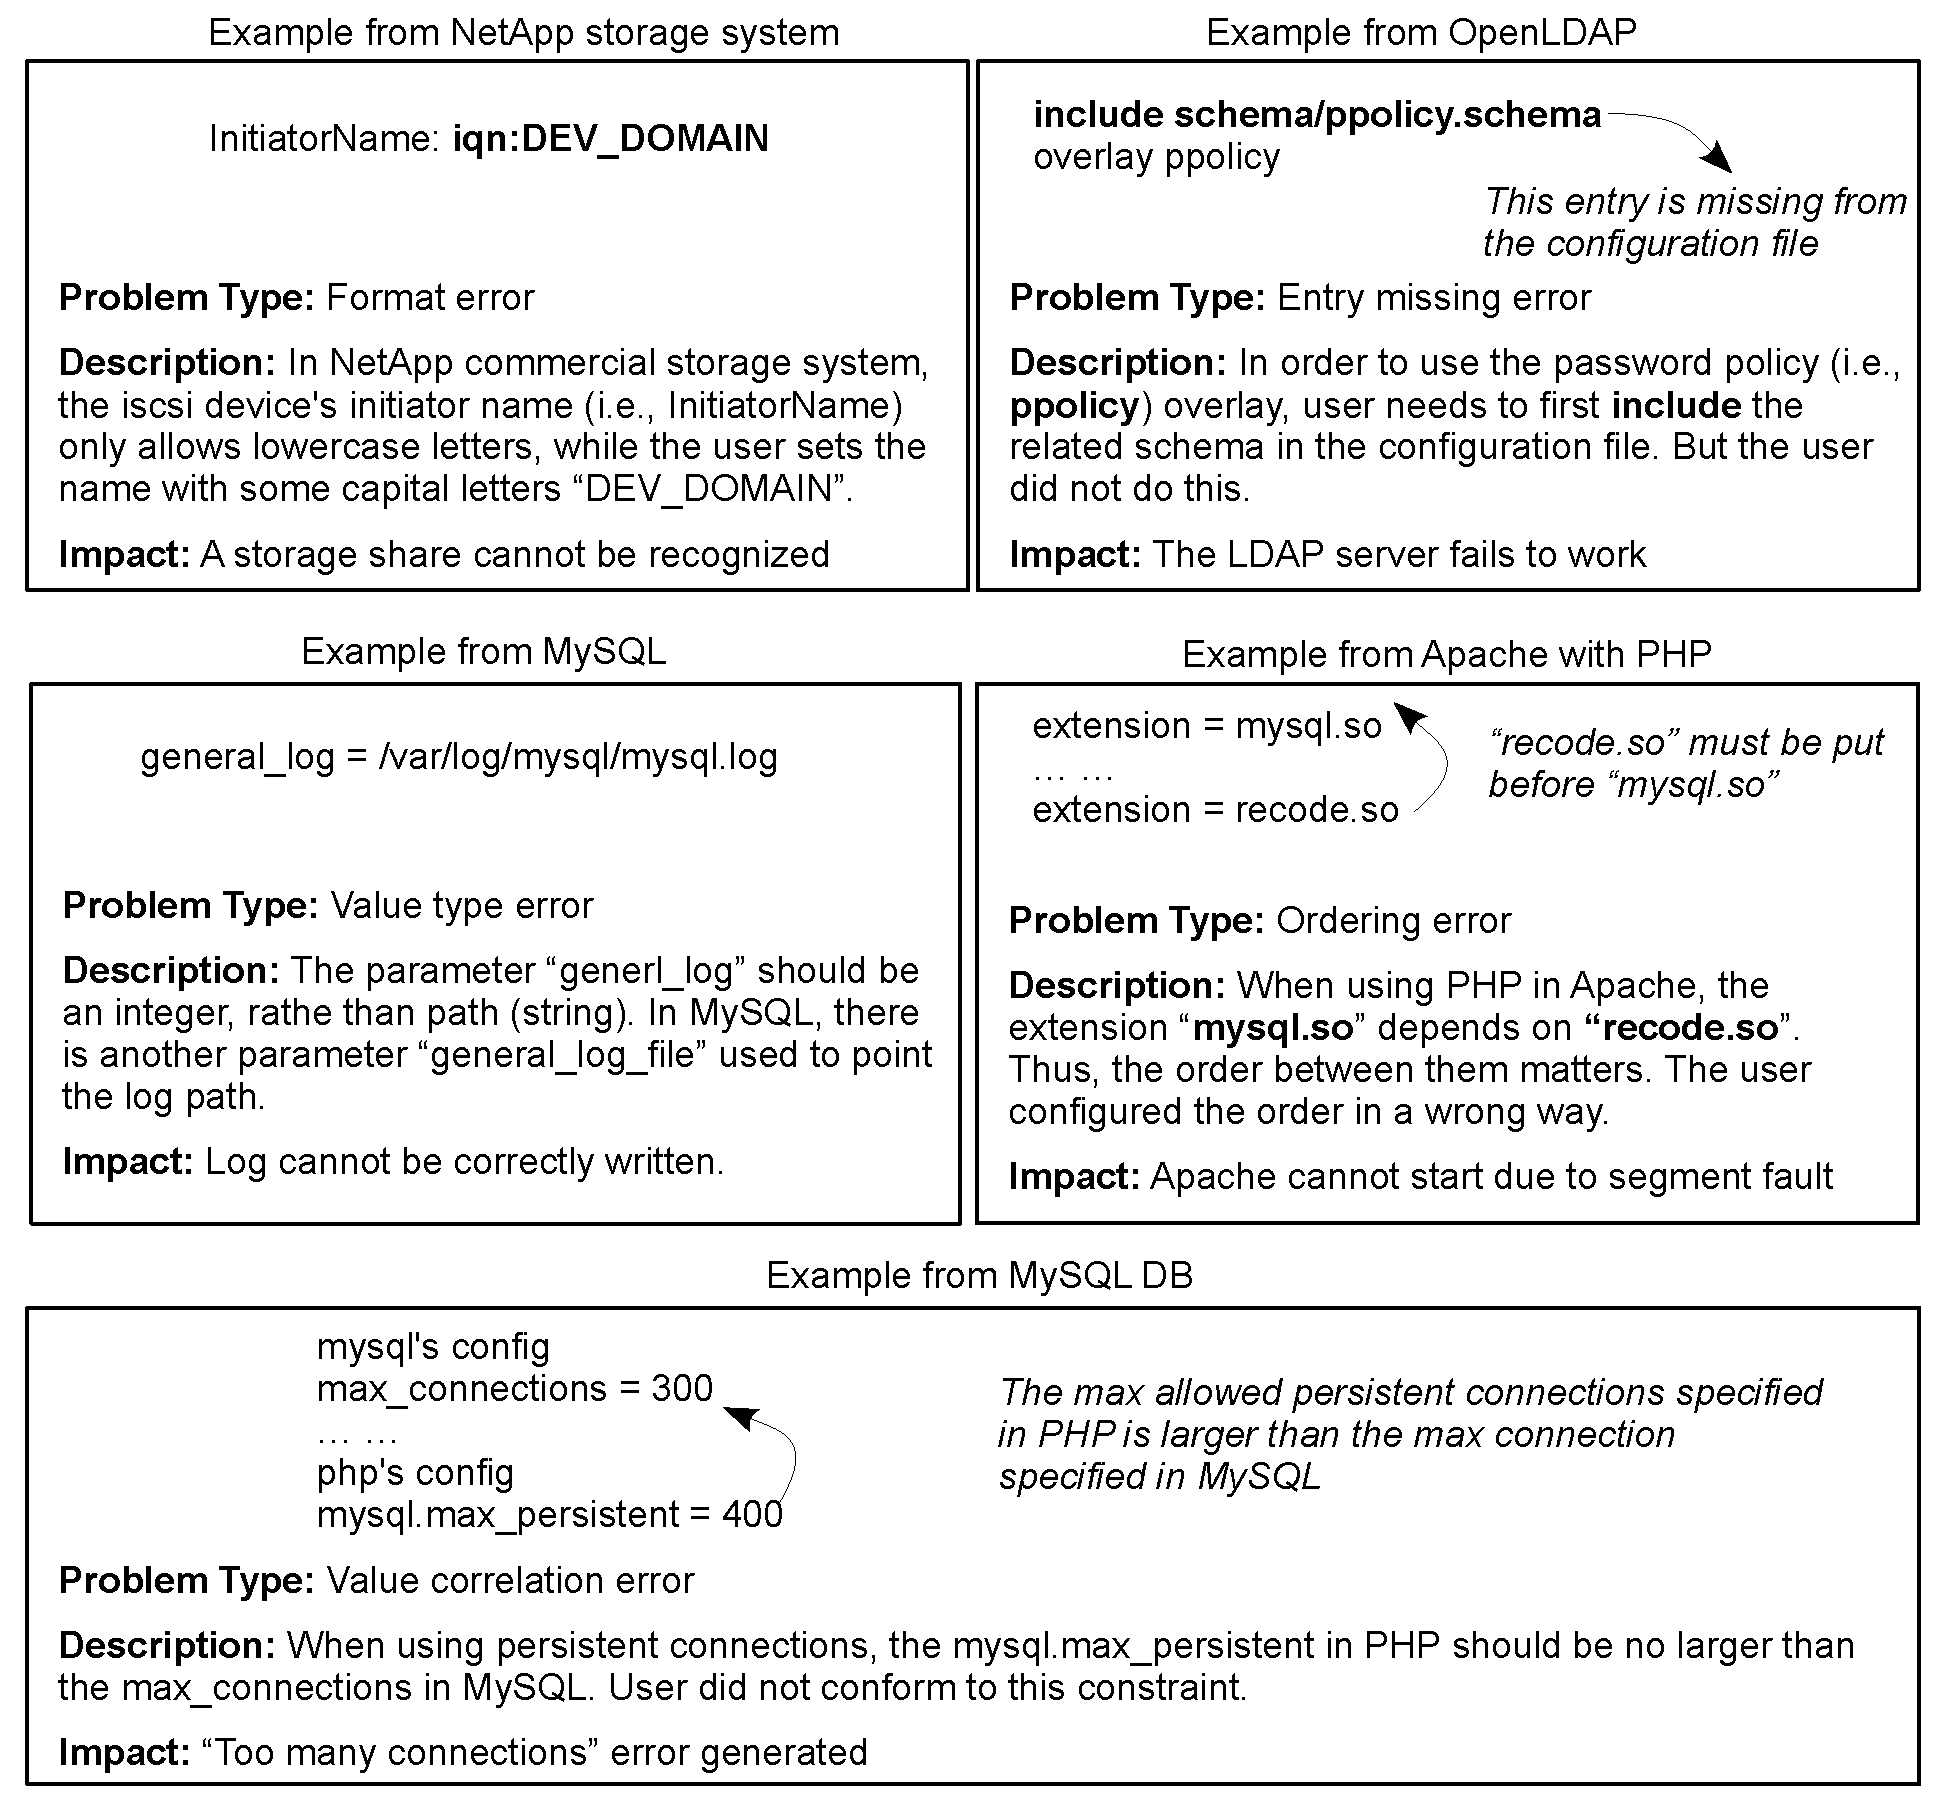
\includegraphics[width=0.98\textwidth]{figs/example}
\caption{Motivating examples. Our target configuration errors are
  classified into five groups. The five examples here correspond to
  these groups, respectively.}
\label{fig-example}
\end{figure}

Fig.~\ref{fig-example} presents misconfiguration examples in real-world
that we aim to address. All the examples are extracted from
misconfiguration issues reported in real-world efforts%
~\cite{yin11anempirical, configdataset}.
We classify our target configuration errors
into five groups: 1) format error; 2) entry missing error; 3) value type
error; and 4) ordering error
The examples in Fig.~\ref{fig-example} correspond to the above four
groups, respectively.

} 


\section{Quantum Types}

Because our type inference is based on machine learning, we cannot be sure that a keyword unambigously has a single type.
This is an issue when we try to learn relational rules between keywords. 
Take the following file in the learning

foo = 300
bar = 300.txt


We want to learn the rule that $foo \in {substring(bar)}$, however using unambigous type inference, we would assign foo type int, and never try to generate a string relation rule for these two keywords.
By assigning foo a quantum type (e.g. ${Int <90\%>, String <10\%>}$), we can now generate rules for both types.

At runtime, when the user wants to check a file we update the probabilities one last time then 'collapse' the quantum type to a concrete type.
If the concrete type collapses to a Int, we consider the rules for ints, and vice versa.

This idea is closely related to exstentially quantified types.


\section{Learning strategy}

A primary concern in any machine learning type task is to minimize false negatives and false positives.
In the context of configuration file verification,
  a false positive is when \app reports an error on a valid confiuration file and
  a false negative is when \app fails to reports an error on an invalid confiuration file.
Too many false positives will cause users to ignore the reported error\cite{}.
However, since the cost of system failure is so high from a misconfiguration, \app propritzes the minimization of false negatives.

While a traditional classififcation learning machine learning approach can reduce both of these situations, there is can generally be no garuntee that all false negatives will be eliminated.
Instead of building classification models over the learning set (such as an SVM), we learn the largest set of rules that all correct configuration files satisfy.
In this way, \app can garuntee that, over the set of rules we consider, there will be no false negatives that could have been caught with the given learning set.
The only case of a false negative can be when there was no evidece of such a rule in the learning set - we cannot generate rules from nothing.
Framed as the question "Is this file valid", \app is complete but not sound. 

That is, taking the following definitions:
\begin{multline*}\\
\text{\{Considered Rules\}} = \forall files \in \text{\{Learning Set\}}, \{ r | r(files) = True \land r \text{ is non-trivial}\}\\
\text{\{Reported Rules\}} = {r | r(userfile)=False } \\
\text{\{True Rules\}} = \{r | \text{ if } r(userfile)=False \text{ then system crash } \land \\
   \exists file \in \text{\{Learning Set\}}, r(file) \text{ is non-trivial}\}
\end{multline*}

We have the following specification of \app.
\begin{multline*}\\
\text{\{True Rules\}} \subseteq \text{\{Considered Rules\}} \\
\forall r \in \text{\{True Rules\}}, if r(userfile)=False then \exists r \in \text{\{Reported Rules\}} \\
\neg \forall r \in \text{\{Reported Rules\}}, r \in \text{\{True Rules\}} \\
\end{multline*}

Another benefit to a rule based approach is that, unlike many classificaton models, \app can actually report the reason for failure, similar to a comiler for a programming language.
This is in contrast to neural nets for example, where we would just get a boolean value, and the mechanics of the system are entirly lost.
Reporting useful errors that specify a point of failure is important to help users fix their misconfigurations.

\section{Intermediate Representation}

Part of the reason configuration file errors are so common is because of the large number of different systems being used on the market.
Rather than proposing a new, unifying, configuration language (so that there would then be n+1 configuration languages), we use in intermediate representation language.
This allows us to reuse all our algorithms over any configuration file that can be convereted to the intermediate representation.
The portability of \app means that with very little intervtion, it can be widely used and adopted.

More grammatically complex languages tend to be harder to translation to an intermediate representation.
While there can be some context senestive structures in configuration files, we found it is easier to design the rule modules (Section \ref{}) to handle learning such structure, rather than encoding it in the intermediate representation.
Additionally, configuration files are generally grammatically simple, consisting mostly of a list of keyword-value pairs.
The keyword is the variable to be used in the system, and the value is the new value for that variable.

To specialize the converter for a particular language, a user must define a new language type, which simply acts as a flag for translation.
If a langauge requires specialized parsing, the user can write such code in the convert function based on pattern matching over the language type.
For example, the user must specify the delimiters of the language (characters for assignment and comments) for their new language. 

\section{Rules}

A core design principle in \app is modularity, so that a user can easily exentend it to their verification needs.
Rather than try to support every type of verification over configuration files, we provide a framework for defining new verfication properties.
We call each verification property a rule, for example the correct ordering of keywords or integer relationships between values.
These rules tend to be pairs of values with a relation.
For instance, an integer relation rule might be that the value of "foo" must be greater than the value of "bar".
It is also important that the rule has some empty value, to state that it is known there is no relation between the values.
This will prevent \app from trying to relearn rules when they have already been refuted.

These rules are represented as a type, where the type must support a particular interface (called a typeclass in Haskell) to be compatible with our system.
The typeclass can support anything that is Foldable, which roughly the user can use any datastructure.
In fact, in our implementation, two rules are implemented with lists, and two others use hashmaps.

\begin{lstlisting}
class Foldable t => Attribute t a where
  learn :: IRConfigFile -> t a
  merge :: t a -> t a -> t a
  check :: t a -> IRConfigFile -> Error
\end{lstlisting} 

The functions of this typeclass will be used, invisibly to the user, to make the overall system run.
As long as the specifications for each function are met, \app can garuntee completness.

\subsection{learn}
  For a single given file in the intermediate representation format, learn the full set of rules on that file.
  By overfitting to each file, we can eventually garuntee the completness of \app.
  The specification of this function is the obvious reduction of the Considered Set definition.

  $\text{learn } file =  \{ r | r(file) = True \land r \text{ is non-trivial}\}$

\subsection{merge}
  Merging the sets of rules from two files to build a new set that is true over both files is the most difficult and important function a rule must implement.
  This is generally implemented as a filter over the union of the two set, but may vary slightly.
  The formal specification of this method is that:
  \begin{multline*}
  \text{merge } Set1 \: Set2= \{r \mid \\
    r \in \text{Set1} \cup \text{Set2} \land \\
    \exists file \forall r' \in \text{Set1} \cup \text{Set2}, r(file) = True \land r'(file) = True \} \\
  \end{multline*}

\subsection{check}
  To check a file by using a rule set, we simply take all the rules that are releveant to the user's file.
  Rules that are relavent are the ones where both parts of the ordering are present.
  We learn the rule set for the user file, and every rule in the learned set must be present in the user file.

\section{Implementation}

\subsection{System}
Since we learn a set of rules on each file in isolation from the other, we have an embarrassing parallel situation.
Haskell allows us to easily take advantage of by using the parallel mapping library, parmap, both for translation to the intermediate representation, and for learning the rules on each file.
\xxx{merge can also be parallelized, but i haven't done it yet and might not get a chance}

\begin{lstlisting}
learnRules :: [ConfigFile Language] -> RuleSet
learnRules fs = let
  fs' = parMap rseq convert fs
  rs = parMap rdeepseq findAllRules fs'
 in
  foldl1 mergeRules rs
\end{lstlisting}

\subsection{Type Error Rules}
This builds a map between keywords and types, using the values as evidence.
see quantum.tex for more
i will write more on this tomorrow.

\subsection{Integer Relation Rules}
we only consider the relations , (==), (<=), (>=) because they are easy to pass aroud (as actual functions) in haskell.
We also committed cardinal since and create an instance for equality over these functions.
instance Eq (Int->Int->Bool) where

With more engineering effort, this could be extened with the use of a SMT solver to create more fine grained relational rules.
From our experience, more specific rule are not really needed for integer relations in configuration files.
However an SMT solver approach would be particularly useful for relations on strings, especially when considering substring relations between filepaths.

\subsection{Ordering and Missing Entry Rules}
These are the simpiliest of all rules, just making a lot of pairs and seeing which pairs continue to appear over the learning set.

There is actually a bit of a catch in ordering though - we are not complete over ordering rules.
This is because only our implementation does not satisfy the specification for the merge function listed above.
The problem arises from the fact the configuration files may have non-unique keywords.
Therefor, in the follwoing file we will derive the valid, but conflicting rules ([client],port) and (port,[client]).
\begin{verbatim}
[client]
port = 3306
[mysqld]
port = 3306
\end{verbatim}
Our implementation of merge removes and conflicting rules for the running set.
By introducing a renaming pass in the initial parsing we may be able to solve this, but have not found a satisfactory solution yet.



\section{Introduction}
\label{sec-intro}

Configuration errors are one of the most important root causes of
today's software system failures~\cite{xu15systems, yin11anempirical}.
For example, Yin {\em et al.}~\cite{yin11anempirical} report
that about 31\% system failures were caused by misconfiguration problems and only 20\% were caused by bugs in program code. 
Misconfigurations, in practice, may result in various
system-wide problems, such as security vulnerabilities, 
application crashes, severe disruptions in software
functionality, and incorrect program executions%
~\cite{zhang14encore, yuan11context, xu13do, xu15hey}.  

While many efforts have been proposed 
to check, troubleshoot, diagnose, and repair configuration errors%
~\cite{attariyan10automating,
su07autobash, whitaker04configuration},
those tools mainly try to understand {\emph{what}} caused the error ---
they are still not on the level of
automatic verification tools used for regular program 
verification~\cite{Leino10Dafny, PiskacWZ14, BobotFMP15}.
Nevertheless, automated verification of configuration 
files would be highly
desirable~\cite{wang04automatic, zhang14encore, xu15systems}.
Two main obstacles why we cannot simply apply the existing automatic 
tools and techniques to verification of configuration files are: 1) a lack
of a specification which would describe properties of configuration files, and 2) a program structure of configuration files -- they
are mainly a sequence of entries assigning some value to system variables. The language in which configuration files are written does 
not adhere to a specific grammar or syntax. In particular,  the
entries in configuration files are untyped. Moreover, there are surprisingly few rules specifying constraints on entries and there
is no explicit structure policy for the entries.

In order to overcome all these obstacles,
researchers have proposed 
statistical analysis and learning based approaches%
~\cite{wang04automatic, zhang14encore, yuan11context}. 
These efforts build checking policies by learning a sample 
data set, rather than explicitly specifying entries' types or rules.
In particular, for each entry in a certain configuration file, 
if it deviates from the common values used in a large collection
of configurations (\ie, the data set for training), it is typically
suspected as a potential configuration error.
However, because these learning 
efforts {\em either} are limited to simplistic 
configuration errors (\eg, type errors and syntax errors), 
{\em or} heavily rely on template-based inference~\cite{zhang14encore}, 
many sophisticated configuration errors, 
\eg, hard to be templated in practice, cannot be detected.
For example, if {\tt extension = mysql.so} appears 
before {\tt extension = recode.so} in PHP configuration file,  
it would lead to a crash error, since the correct ordering 
should be {\tt extension = recode.so} before 
{\tt extension = mysql.so}~\cite{yin11anempirical};
however, such an error cannot be detected by existing
learning efforts, since it is hard to build a template for this
error~\cite{xu15systems}.

%Offering automatic verification to configuration files -- like
%what we did to programs -- has been advocated as a reasonable means
%to check the correctness of configuration files of interest.
%Nevertheless, it is still an open problem, because 
%1) software configurations are typically written in poorly structured 
%and untyped languages, and 2) writing specifications or constraints
%for configuration verification is non-trivial in practice.

In order to truly achieve automatic configuration verification,
we argue that we need to leverage a collection of more powerful learning 
algorithms (not necessarily depending on templates) to derive 
a more sophisticated language model (with abundant rules covering
tricky configuration errors), and then check the configuration files
of interest through the learned language model.

Based on the above argument, 
this paper presents \app, the first automatic verification framework
for general software configurations.
In particular, \app's workflow to verifying a given configuration file
could be looked as a three-step methodology.
First, \app analyzes a dataset containing sample configuration files,
thus generating a well-structured and probabilistically-typed 
intermediate representation.
Second, \app derives rules and constraints by analyzing
the intermediate representations, thus building a language model.
Finally, \app uses the resulting language model
to verify the given configuration file and detect potential errors.
Compared with previous efforts,
\app does not necessarily rely on users' templates, 
and is capable of detecting more tricky configuration errors that
cannot be identified by existing work (details in $\S$\ref{sec-motiv}). 

Building such an automatic verification framework for
configuration files, nevertheless, requires addressing several challenges. 
First, in order to formulate a correct language model, 
we need to infer each entry's type in a given configuration file;
however, the type of a variable cannot always be fully determined 
from a single value. 
For example, an entry {\tt foo = MAX\_SIZE} is most likely
an integer rather than string; however, existing type inference 
work would report this is an error, because foo should be assigned
an integer~\cite{zhang14encore}. We address this problem by introducing 
so called {\emph{probabilistic types}}.
Rather than assigning only one variable to a single type, 
we assign several types with their probability distributions. 
The entry in the above example might be assigned 
a probabilistic type like 
{\tt \{foo, MAX\_SIZE, [(Int, 60\%), (String, 40\%)]\}}.
With such probabilistic types in hand,
we can generate a more accurate language model,
thus significantly improving our checking capability.

Second, without template, how to learn rules and constraints present
a difficult. \ennan{Here, we need to add one-paragraph description 
to illustrate how we learn rules without templates, 
or why we say our learning results are better than existing
learning approach, \eg, EnCore.}

\com{First, given the fact that 
different systems' configuration files use various representations, 
the cost of introducing a completely new configuration
language (or representation) to instead of all these existing format looks 
like an impractical goal. This is not only because administrators need 
to learn this new language, but also changes existing system
infrastructure to support such a new language. 
In order to avoid the above issues, we propose a representation,
which is a type-based representation and 
much more structured than existing configuration format, 
but use it as an intermediate layer. We, at the same time,
develop many pluggable parsers
that can transform different systems' configuration representations
into our proposed intermediate representation for the post process.}

From a practical perspective, 
\app introduces no additional burden 
to the users: they can simply use \app to check for errors in their
configuration files. However, they can also easily extend the framework
themselves. The system is designed to be highly modular. If there is a
class of rules that \app is not currently learning, the user can develop
their own templates and learners for that class. The new learner can be
added to \app and this way it can check additionally a new set of
errors.

Our \app prototype still has a few limitations:
for example, we cannot handle configuration errors that can be only
triggered in system execution time.
Nevertheless, we believe \app may suggest a practical path
toward automatic and modular language-based configuration verification.
To summarize, this tool paper makes the following contributions:

\com{
Finally, from a systems perspective this is the first approach that {\emph{proactively}} checks 
 the correctness of configuration files. All previous work
~\cite{xu15systems,zhang14encore,yuan11context, wang04automatic,attariyan10automating,
su07autobash,whitaker04configuration} tries to identify the problem after the
failure occurred. Our approach isolates potential errors before the system failure occurs, e.g. before the installation. We can also see \app as a tool that can run in conjunction with existing tools. Pre-analyzed configuration files are already free from language-based errors, and this way the workloads of post-failure forensics at the runtime
is significantly reduced, thus making these tools truly practical.
}


\begin{enumerate}

\item We propose the first automatic configuration verification
framework, \app, that can learn a language model from an example set of 
correct configuration files, and then uses this language model to verify 
interested configuration files.
 
\item \app proposes probabilistic types to assign a confidence 
distribution over a set of types to each entry, 
while generating the intermediate representation. 

\item \app employs a collection of machine learning algorithms to 
enable powerful rule and constraint inference without the assistance 
from any pre-defined templates.

\item \app is capable of detecting various tricky errors that cannot
be detected by previous efforts,
including ordering errors, fine-grained value correlation errors, 
entry missing errors, and environment related errors. 

\item We implement a \app prototype and evaluate it by
conducting comprehensive experiments.

\end{enumerate}

%\section{Motivating Examples}
\label{sec-motiv}

In this section we present the capability of \app through 
detecting errors in several real-world misconfiguration examples. 
These examples were non-trivial configuration errors
that were reported on StackOverflow~\cite{stackoverflow},
a popular question and answer website for programmers and administrators. 
%To better understand these problems, 
%we explored and analyzed misconfigurations 
%on a large number of user forums and on-line discussion sites.

\para{Example~1: Ordering error} 
Ordering errors were reported by Yin {\em et al.}~\cite{yin11anempirical} and our first
example illustrates how ordering errors can cause a system to crash. When a user configures PHP 
to run with the
Apache HTTP Server, most likely the user will take some already existing configuration files and adapt them
to suit her needs. The configuration file might contain, among others, 
the following lines:

\begin{lstlisting}[language=C, xleftmargin=.01\textwidth]
    extension = mysql.so
        ...
    extension = recode.so
\end{lstlisting}

This configuration file will cause the Apache server to 
fail to start due to a segmentation fault error. 
This is because, when using PHP in Apache, the extension {\tt mysql.so} 
depends on {\tt recode.so}, and their relative ordering
is crucial. 
We call the above example of a misconfiguration file
an {\em ordering error}.
Yin {\em et al.} report that ordering errors widely exist in
many system configurations, \eg, PHP and MySQL,
and typically lead to multiple system crash events.
However, no existing tool can effectively solve 
or detect this problem~\cite{zhang14encore, xu15systems, xu13do}.

By invoking \app, the user can detect such a configuration error.
In particular, \app reports that {\tt recode.so} 
should appear before {\tt mysql.so}, as shown
below:
 
\begin{lstlisting}[language=C, xleftmargin=.01\textwidth]
    ORDERING ERROR: Expected "extension=recode.so"
    BEFORE "extension=mysql.so"
\end{lstlisting} 

%TODO would be nice to have these as subsection or somehow be able to ref specific examples
\para{Example~2: Fine-grained integer correlation error}
\label{ex:fine}
Our second misconfiguration example~\cite{correlation} 
comes from a discussion on StackOverflow.
The user has configured her MySQL as in the following:

\begin{lstlisting}[language=C, xleftmargin=.01\textwidth]
    key_buffer_size = 384M
    max_heap_table_size = 128M
    max_connections = 64
    thread_cache_size = 8
        ...
    sort_buffer_size = 32M
    join_buffer_size = 32M
    read_buffer_size = 32M
    read_rnd_buffer_size = 8M
        ...
\end{lstlisting} 

The user complains that her MySQL load was very high, 
causing the website's
response speed to be very slow.
In this case, {\tt key\_buffer\_size} is used by all the threads
cooperatively, while {\tt join\_buffer} and {\tt sort\_buffer} are 
created by each thread for private use; thus, {\tt key\_buffer\_size},
\ie, the maximum amount of used key buffer, should be larger than 
{\tt join|sort\_buffer\_size} * {\tt max\_connections}. 
In the above example, however, it does not hold. 

If we run \app on this configuration file, \app  would return:

\begin{lstlisting}[language=C, xleftmargin=.01\textwidth]
  FINE GRAINED INTEGER RELATION ERROR:
  Expected "max_connections" * "sort_buffer_size"
               =< "key_buffer_size"
\end{lstlisting} 

The above example is a complex integer correlation, which implicitly
includes a computational correlation among different entries
in the configuration file.
We call these complex integer correlations as 
{\em fine-grained integer correlations}. 
Our tool can detect simple integer correlation---one entry's
value should have a certain correlation with another entry's 
value---as well.
For example, in MySQL, the value of {\tt max\_connections} 
should be higher than {\tt mysql.max\_persistent}.
While few existing tools~\cite{yin11anempirical, zhang14encore}
can detect the simple integer correlation errors,
to the best of our knowledge, \app is the first effort capable of
detecting fine-grained integer correlation problems.

\para{Example~3: Missing entry error} 
Many critical system outages result from the fact that an important
entry was missing from the configuration file. 
We call such a problem a {\em missing entry error}.
In a public misconfiguration dataset~\cite{configdataset},
many MySQL failure reports were caused by
missing entry errors.
Below is a real-world missing entry error example~\cite{yin11anempirical}:
when a user wants to use OpenLDAP to enable her directory access
protocol, she needs to use the password policy overlay. This is usually
achieved via the following entries in the OpenLDAP configuration file:

\begin{lstlisting}[language=C, xleftmargin=.01\textwidth]
    include schema/ppolicy.schema
    overlay ppolicy
\end{lstlisting} 

When using the password policy overlay in OpenLDAP, 
users must first include the related schema.
Leaving out the {\tt include schema/ppolicy.schema} entry, 
as done by many users~\cite{yin11anempirical}, 
causes the failure of LDAP. 
If the user runs \app on such a misconfiguration file,
\app would return:

\begin{lstlisting}[language=C, xleftmargin=.01\textwidth]
    MISSING ENTRY ERROR: Expected "overlay" "ppolicy"
    in the same file: "include" "schema/ppolicy.schema"
\end{lstlisting} 

\para{Example~4: Type errors} 
Many system availability problems are caused by 
assigning incorrect type of values to some key in configuration
files. Consider the following real-world misconfiguration
file~\cite{typeerror}: 
a user tries to install MySQL and she needs to initiate the path
of the log information generated by MySQL.
This user puts the following entry assignment in her MySQL
configuration file: 

\begin{lstlisting}[language=C, xleftmargin=.01\textwidth]
    slow-query-log = /var/log/mysql/slow.log
\end{lstlisting} 

Unbeknowest to this user, the entry ``slow-query-log'' should be an 
integer, not a string. This misconfiguration will lead to 
MySQL fails to start~\cite{querylog}. In MySQL, there is another entry 
named ``slow-query-log-file'' used to specify the log path.
With \app, this user can get the following result:

\begin{lstlisting}[language=C, xleftmargin=.01\textwidth]
    TYPE ERROR: Expected a Int with P=1.0 for
    "slow-query-log"
\end{lstlisting} 

%The above result means that we need to assign an integer value to
%the entry ``general\_log''. 

\section{Quantum Types}

Because our type inference is based on machine learning, we cannot be sure that a keyword unambigously has a single type.
This is an issue when we try to learn relational rules between keywords.
Take the following file in the learning

foo = 300
bar = 300.txt

We want to learn the rule that $foo \in {substring(bar)}$, however using unambigous type inference, we would assign foo type int, and never try to generate a string relation rule for these two keywords.
By assigning foo a quantum type (e.g. ${Int <90\%>, String <10\%>}$), we can now generate rules for both types.

At runtime, when the user wants to check a file we update the probabilities one last time then 'collapse' the quantum type to a concrete type.
If the concrete type collapses to a Int, we consider the rules for ints, and vice versa.

This idea is closely related to exstentially quantified types.

Here is what we know:
- When parsing unstructured (plaintext) data, we may not be given, or able to fully determine, the type of a value.
- We can guess types based on regular expressions over a value.*
- Guessing a concrete type can be overly restrictive. In ConfigC is prematurely pruning the rule search.
- By guessing a set of types with probabilities, we can continously update the distribution, and decide on a concrete type later when we have more information.

Here are things we need to know:
- In ConfigC, we are building probabilistic types, but only operate (i.e. build rules) over the component, concrete types. Can we also operate over probabilistic types and maintain type safety? Fundamentally, we ask "What do we need to add to the simply typed lambda calculus to express probabilistic types?"
- How is this related to existentially quantified types (another "heterogeneous collection" type). Can/should we use this for an implementation?
- How is this related to a value-level probabilistic lambda calculus (where probabilities are on value).
- Does this type system need to be tied to the specific machine learning techniques used in infering types?
- Can we do inference based on more interesting things than just regular expression (something a bit like **, maybe which types generate better rules)
- We might also ask, is there any good reason to operate over probabilistic types? What are other situations when we might need/encounter probabilistic types?

*This focuses mostly on using regular expression to infer concrete types. http://people.csail.mit.edu/rishabh/papers/popl16-semantic.pdf
** http://conf.researchr.org/event/POPL-2016/popl-2016-papers-estimating-types-in-binaries-using-predictive-modeling


\section{\app Design}

\xxx{
\app Design: 
  \begin{itemize}
  \item Present an architecture of \app with a fig. Briefly describe 
    how it works (step by step).
  \item Detail learner part
  \item Merge
  \item Check 
  \item Limitations
  \end{itemize}
}

\section{Learning strategy}

A primary concern in any machine learning type task is to minimize false negatives and false positives.
In the context of configuration file verification,
  a false positive is when \app reports an error on a valid confiuration file and
  a false negative is when \app fails to reports an error on an invalid confiuration file.
Too many false positives will cause users to ignore the reported error\cite{}.
However, since the cost of system failure is so high from a misconfiguration, \app propritzes the minimization of false negatives.

While a traditional classififcation learning machine learning approach can reduce both of these situations, there is can generally be no garuntee that all false negatives will be eliminated.
Instead of building classification models over the learning set (such as an SVM), we learn the largest set of rules that all correct configuration files satisfy.
In this way, \app can garuntee that, over the set of rules we consider, there will be no false negatives that could have been caught with the given learning set.
The only case of a false negative can be when there was no evidece of such a rule in the learning set - we cannot generate rules from nothing.
Framed as the question "Is this file valid", \app is complete but not sound. 

That is, taking the following definitions:
\begin{multline*}\\
\text{\{Considered Rules\}} = \forall files \in \text{\{Learning Set\}}, \{ r | r(files) = True \land r \text{ is non-trivial}\}\\
\text{\{Reported Rules\}} = {r | r(userfile)=False } \\
\text{\{True Rules\}} = \{r | \text{ if } r(userfile)=False \text{ then system crash } \land \\
   \exists file \in \text{\{Learning Set\}}, r(file) \text{ is non-trivial}\}
\end{multline*}

We have the following specification of \app.
\begin{multline*}\\
\text{\{True Rules\}} \subseteq \text{\{Considered Rules\}} \\
\forall r \in \text{\{True Rules\}}, if r(userfile)=False then \exists r \in \text{\{Reported Rules\}} \\
\neg \forall r \in \text{\{Reported Rules\}}, r \in \text{\{True Rules\}} \\
\end{multline*}

Another benefit to a rule based approach is that, unlike many classificaton models, \app can actually report the reason for failure, similar to a comiler for a programming language.
This is in contrast to neural nets for example, where we would just get a boolean value, and the mechanics of the system are entirly lost.
Reporting useful errors that specify a point of failure is important to help users fix their misconfigurations.

\section{Intermediate Representation}

Part of the reason configuration file errors are so common is because of the large number of different systems being used on the market.
Rather than proposing a new, unifying, configuration language (so that there would then be n+1 configuration languages), we use in intermediate representation language.
This allows us to reuse all our algorithms over any configuration file that can be convereted to the intermediate representation.
The portability of \app means that with very little intervtion, it can be widely used and adopted.

More grammatically complex languages tend to be harder to translation to an intermediate representation.
While there can be some context senestive structures in configuration files, we found it is easier to design the rule modules (Section \ref{}) to handle learning such structure, rather than encoding it in the intermediate representation.
Additionally, configuration files are generally grammatically simple, consisting mostly of a list of keyword-value pairs.
The keyword is the variable to be used in the system, and the value is the new value for that variable.

To specialize the converter for a particular language, a user must define a new language type, which simply acts as a flag for translation.
If a langauge requires specialized parsing, the user can write such code in the convert function based on pattern matching over the language type.
For example, the user must specify the delimiters of the language (characters for assignment and comments) for their new language. 

\section{Rules}

A core design principle in \app is modularity, so that a user can easily exentend it to their verification needs.
Rather than try to support every type of verification over configuration files, we provide a framework for defining new verfication properties.
We call each verification property a rule, for example the correct ordering of keywords or integer relationships between values.
These rules tend to be pairs of values with a relation.
For instance, an integer relation rule might be that the value of "foo" must be greater than the value of "bar".
It is also important that the rule has some empty value, to state that it is known there is no relation between the values.
This will prevent \app from trying to relearn rules when they have already been refuted.

These rules are represented as a type, where the type must support a particular interface (called a typeclass in Haskell) to be compatible with our system.
The typeclass can support anything that is Foldable, which roughly the user can use any datastructure.
In fact, in our implementation, two rules are implemented with lists, and two others use hashmaps.

\begin{lstlisting}
class Foldable t => Attribute t a where
  learn :: IRConfigFile -> t a
  merge :: t a -> t a -> t a
  check :: t a -> IRConfigFile -> Error
\end{lstlisting} 

The functions of this typeclass will be used, invisibly to the user, to make the overall system run.
As long as the specifications for each function are met, \app can garuntee completness.

\subsection{learn}
  For a single given file in the intermediate representation format, learn the full set of rules on that file.
  By overfitting to each file, we can eventually garuntee the completness of \app.
  The specification of this function is the obvious reduction of the Considered Set definition.

  $\text{learn } file =  \{ r | r(file) = True \land r \text{ is non-trivial}\}$

\subsection{merge}
  Merging the sets of rules from two files to build a new set that is true over both files is the most difficult and important function a rule must implement.
  This is generally implemented as a filter over the union of the two set, but may vary slightly.
  The formal specification of this method is that:
  \begin{multline*}
  \text{merge } Set1 \: Set2= \{r \mid \\
    r \in \text{Set1} \cup \text{Set2} \land \\
    \exists file \forall r' \in \text{Set1} \cup \text{Set2}, r(file) = True \land r'(file) = True \} \\
  \end{multline*}

\subsection{check}
  To check a file by using a rule set, we simply take all the rules that are releveant to the user's file.
  Rules that are relavent are the ones where both parts of the ordering are present.
  We learn the rule set for the user file, and every rule in the learned set must be present in the user file.

\section{Implementation}

\subsection{System}
Since we learn a set of rules on each file in isolation from the other, we have an embarrassing parallel situation.
Haskell allows us to easily take advantage of by using the parallel mapping library, parmap, both for translation to the intermediate representation, and for learning the rules on each file.
\xxx{merge can also be parallelized, but i haven't done it yet and might not get a chance}

\begin{lstlisting}
learnRules :: [ConfigFile Language] -> RuleSet
learnRules fs = let
  fs' = parMap rseq convert fs
  rs = parMap rdeepseq findAllRules fs'
 in
  foldl1 mergeRules rs
\end{lstlisting}

\subsection{Type Error Rules}
This builds a map between keywords and types, using the values as evidence.
see quantum.tex for more
i will write more on this tomorrow.

\subsection{Integer Relation Rules}
we only consider the relations , (==), (<=), (>=) because they are easy to pass aroud (as actual functions) in haskell.
We also committed cardinal since and create an instance for equality over these functions.
instance Eq (Int->Int->Bool) where

With more engineering effort, this could be extened with the use of a SMT solver to create more fine grained relational rules.
From our experience, more specific rule are not really needed for integer relations in configuration files.
However an SMT solver approach would be particularly useful for relations on strings, especially when considering substring relations between filepaths.

\subsection{Ordering and Missing Entry Rules}
These are the simpiliest of all rules, just making a lot of pairs and seeing which pairs continue to appear over the learning set.

There is actually a bit of a catch in ordering though - we are not complete over ordering rules.
This is because only our implementation does not satisfy the specification for the merge function listed above.
The problem arises from the fact the configuration files may have non-unique keywords.
Therefor, in the follwoing file we will derive the valid, but conflicting rules ([client],port) and (port,[client]).
\begin{verbatim}
[client]
port = 3306
[mysqld]
port = 3306
\end{verbatim}
Our implementation of merge removes and conflicting rules for the running set.
By introducing a renaming pass in the initial parsing we may be able to solve this, but have not found a satisfactory solution yet.


\section{Implementation and Evaluation}
\label{sec:eval}

We have implemented a tool, \app, and evaluated it based on real-world configuration files taken from Github.
\app is written in Haskell and is available open source at \textit{url redacted for anonymity}.
Thanks to the Haskell's powerful type system, the implementation can easily be extended with new rule classes or applied to different configuration languages with minimal change to the rest of the code base.
A user only needs to provide the functions for the rule interface (a typeclass in Haskell) to 1) learn relations from a single file 2) merge two sets of rules and 3) check a file given some set of rules.

\subsection{Evaluation}

To evaluate our \app prototype, we require a separate training set and test set. 
For our training set, \trainingSet, we use a preexisting set of 256 
industrial MySQL configuration files collected in previous configuration 
analysis work~\cite{configdataset}.
This is an unlabeled training set, though most of the files have some errors.
For our test set, we collected 1000 MySQL configuration files 
from Github, and filtered the incorrectly formatted files out for a final 
total of 973 files.
In our evaluation, we focus on MySQL for comparability of results, but \app can handle any configuration language (that can be parsed to the intermediate representation from Sec.~\ref{sec:trans}).

We report the number of rules learned from the training set and the number of errors detected in the test set in Table~\ref{table:learning}.
One interesting note is that without probabilistic types we learned 327 fine grained rules and detected 1367 errors.
By introducing probabilistic types, we remove 114 incorrect rules and thereby remove 1023 false positives.
We are guaranteed these are all false positives since there cannot be a correct rule of relating the types $size*size$ and $size$ because of the semantic interpretation of the $size$ units.

We also provide the support and confidence thresholds, $t_s, t_c$, used in this evaluation.
These number can be adjusted by the user as a slider to control the level of assurance that their file is correct.
Since these settings depend on both the user preference and training set quality, we simply choose values for which \app reports reasonably sized output.
This is a determined by the user by examining the rule set output over the training set.
Following common practice from association rule learning, initial values for support are confidence are generally 10\% and 90\% respectively.

We record the histogram of errors across the test set in Figure~\ref{fig:histo}.
This is intuitively an expected result from randomly sampling Github - most repositories will have few errors, with an increasingly small number of repositories having many errors.

\begin{figure}[h]
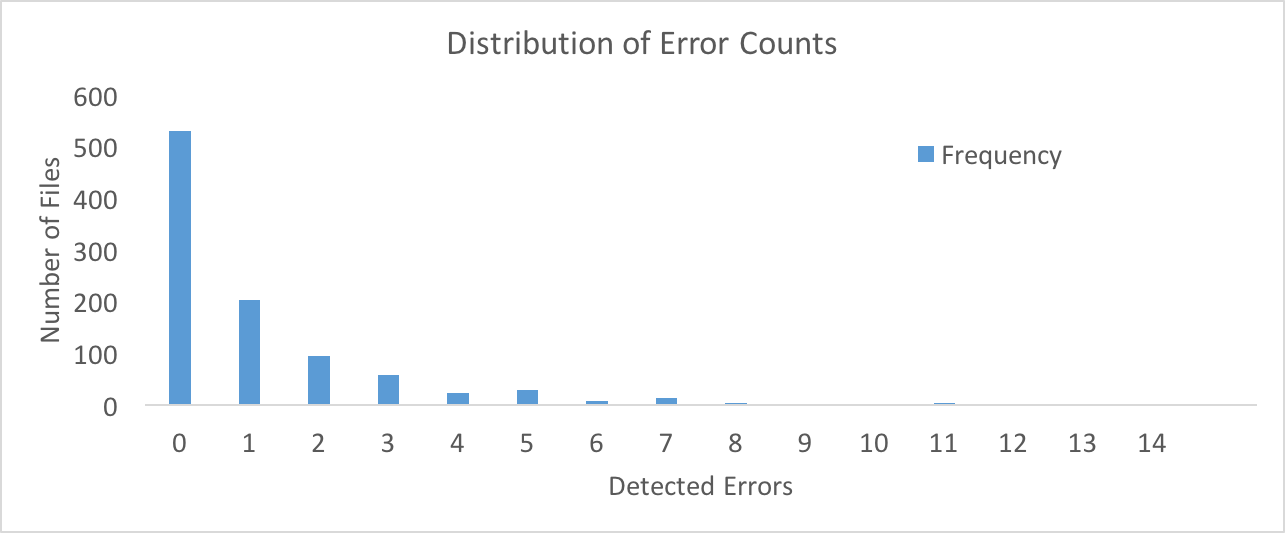
\includegraphics[width=\textwidth]{figs/histogram.png}
\caption{Histogram of errors - 14 errors were detected in 1 file}
\label{fig:histo}
\end{figure}

\begin{table}[h]
\centering
\caption{Results of \app}
\label{table:learning}
\setlength{\tabcolsep}{0.5em}
\begin{tabular}{|c|c|c|c|c|}
\hline
{\bf Class of Error } & {\bf \# Rules Learned} & {\bf \# Errors Detected} & {\bf Support} & {\bf Confidence}\\ 
\hline
\hline
Order        & 13  & 62   & 6 \%  & 94 \% \\ 
Missing      & 53  & 55   & 2 \%  & 71\% \\ 
Type         & 92  & 389  & 12 \% & 70\%  \\ 
Fine-Grain   & 213 & 324  & 24 \% & 91\%  \\ 
Coarse-Grain & 97  & 237  & 10 \% & 96\% \\ 
\hline 
\end{tabular}
\end{table}

The errors reported may have varying impacts on the system, ranging from failing to start, runtime crash, or performance degradation.
However, since \app is a probabilistic system, it is also possible that some errors are false positives, a violation of the rule has no effect on the system.
Note that in contrast to program verification, we do not have an oracle for determining if a reported error is a true error or a false positive.
While we can run a program to determine the effect a specification has on the success of compiling/running the program, no such test exists for configuration files.
Because configurations are dependent on the rest of the system (\ie, the available hardware, the network speed, and the usage patterns), we cannot simulate the all conditions to determine if a reported error will cause system failure.
As evidenced by Example~\ref{ex:fine}, some misconfigurations will only cause greater than expected performance degradation, and only under particular traffic loads.
In light of this, the definition of a true error is necessarily imprecise.

Although we cannot identify false positives, we can identify true positives by examining online forums, like StackOverflow.
On these forums we find reports that particular configuration settings have caused problems on real-world systems.
Furthermore, any error for which we can find evidence online is likely to be more problematic than errors that do not have an online record, 
  using the reasoning that this error has caused enough problems for people to seek help online.
In this case, we would like \app to sort the errors by their importance or potential severity.
To achieve this sorting we use the rule graph analysis metric described in Sec.~\ref{sec:ruleorder}.

To estimate the impact of this metric, we track the rank of known true positives with, and without, the augmented rule ordering in Table~\ref{table-casestudy}.
For this table, we picked the known true positive rules, listed in the Errors column, and pick configuration files in the test set that have these errors.
We picked 3 files for each true positive by choosing the files with the highest number of total reported errors in order to clearly observe the effects of our optimizations.
Although this gives a more clear picture of the effect of our optimizations, it results in a slightly inflated false positive rate.

We test the following conditions; just rule graph analysis (RG) to sort the errors, just probabilistic types to filter the rules (PT), and both optimizations at the same time (RG $\land$ PT).
For each entry we list X/Y, where X is the rank of the known true positive, and Y is the total number of errors found in that file.


\newcommand{\tablewidth}{6cm}
\definecolor{Gray}{gray}{0.80}
\newcolumntype{g}{>{\columncolor{Gray}}c}


\begin{table*}[tbp]
\centering
\caption{Sampled misconfiguration files for error detection evaluation.}
\label{table-casestudy}
\setlength{\tabcolsep}{0.5em}
\begin{footnotesize}
\begin{tabular}{|c|c|c|g|g|c|}
\hline
{\bf Errors} & {\bf URLs} & {\bf None} & {\bf PA} & {\bf PT} & {\bf PT$\land$ PA}\\ 
\hline
\hline
\multirow{3}{*}{\parbox{\tablewidth} {\scriptsize ORDERING ERROR: Expected ``innodb\_data\_home\_dir'' BEFORE ``innodb\_data\_file\_path''} }
& url & 12/12 & 3/12 & 5/5 & 3/5 \\
& url & 11/11 & 2/11 & 3/3 & 3/3 \\ 
& url & 9/9   & 3/9  & 4/4 & 3/4 \\ 
\hline

\multirow{3}{*}{\parbox{\tablewidth} {\scriptsize MISSING ERROR: Expected ``key\_buffer'' WITH [isamchk]} }
& url & 6/10 & 2/10 & 2/4 & 2/4 \\ 
& url & 2/3 & 3/3 & 2/3 & 3/3 \\
& url & 2/3 & 3/3 & 2/2 & 3/3 \\  
\hline

\multirow{3}{*}{\parbox{\tablewidth} {\scriptsize TYPE ERROR: Expected an integer for “slow\_query\_log”}}
& url & 32/34 & 1/34 & 5/7   & 1/7 \\ 
& url & 9/20  & 2/20 & 10/11 & 2/11 \\  
& url & 9/19  & 2/19 & 10/11 & 2/11 \\
\hline

\multirow{3}{*}{\parbox{\tablewidth} {\scriptsize FINE GRAINED ERROR: Expected \\ ``max\_connections'' * ``sort\_buffer\_size'' $\geq$ ``key\_buffer\_size''}}
& url & 30/34 & 18/24 & 6/7 & 3/7 \\ 
& url & 23/25 & 9/25  & 8/9 & 3/9 \\  
& url & 20/23 & 14/23 & 6/7 & 5/7 \\
\hline

\multirow{3}{*}{\parbox{\tablewidth} {\scriptsize INTEGER CORRELATION ERROR: Expected ``max\_allowed\_packet'' $<$ ``innodb\_buffer\_pool\_size''} }
& url & 29/32 & 8/32 & 11/14 & 4/14 \\ 
& url & 22/23 & 2/23 & 9/10  & 2/10 \\  
& url & 10/12 & 4/12 & 4/4   & 2/4 \\
\hline

\end{tabular}
\end{footnotesize}
\end{table*}




\subsection{False Positive Rate}

Because \app detects complex and subtle misconfigurations that, for example, may cause performance degradation in a high traffic load, false positives are system and use-case dependent and therefore ill-defined.
However, we report an estimation of the false positive rate for comparison to other tools.
To estimate a false positive rate, we asked two industry experts, one from MongoDB and one from Microsoft, to independently classify all errors from Table~\ref{table-casestudy}.
For each unique error reported in Table~\ref{table-casestudy} (a total of 70 unique errors), the expert was asked to classify the error as: definitely false positive, potential true positive, or definitely true positive. 
The MongoDB expert rated 13/70 errors as definitely false positives. 
The Microsoft expert rated 8/70 errors as definitely false positives. 
The similarity between experts is suggestive that these are approximately correct classifications.

The resulting false positive rate is then estimated to be 11\%-18\%.
This is in the range of existing work, for example in the EnCore tool, which had a false positive rate of 13\%,21\%,32\% for MySQL, Apache, and PHP respectively~\cite{encore}.
We note again that as opposed to a tool like EnCore, which is used mainly to detect initialization errors, thanks to the complex relations that can be learned, \app also learns misconfigurations causing runtime performance degradation.
This means \app generates a larger rule set, and false positives cannot be guaranteed, \ie there may be some environment conditions that will cause a ``false'' positive to become a true positive.

In contrast, a true positive can be confirmed as such based on evidence of unwanted system behavior.
The errors listed in Table~\ref{table-casestudy} are confirmed true positives, evidenced by posts on help forums.
\app detected and reports these errors in the 15 code repositories listed in the URL column of Table~\ref{table-casestudy}. 
These are real-world configuration files that contain errors that may be unknown to the maintainers of the repositories.
%The errors were not submitted as patches to the repository owners, since it is possible the owner of the repository has a user case for this configuration file that will not trigger the unwanted behavior.

\subsection{Runtime Performance}
We also evaluate the speed of \app.
Generally, once a set of rules has been learned, it is not necessary to rerun the learner.
However, we have only used \app to build rules for MySQL, but any configuration language can be analyzed with \app given a training set, which requires rerunning the learner.
Additionally, in an industrial setting, the available training set may be much larger than ours, so is important that the learning process scales.
We see in Table~\ref{table:training} that \app scales roughly linearly.

We compare \app to prior work in configuration verification, ConfigC~\cite{santolucitoCAV}.
ConfigC scales exponentially because the learning algorithm assumes a completely correct training set, and learns every derivable relation.
With \app, we instead only process rules that meet the required support and confidence, reducing the cost of resolving to a consistent set of rules. 
The times reported in Table~\ref{table:training} were run on four cores of a Kaby Lake Intel Core i7-7500U CPU @ 2.70GHz on 16GB RAM and Fedora 25.

\begin{table}[h!]
\centering
\caption{Time for training over various training set sizes}
\label{table:training}
\setlength{\tabcolsep}{1em}
\begin{tabular}{|c|c|c|}
\hline
{\bf \# of Files for Training} & {\bf ConfigC (sec)} & {\bf \app (sec)}\\ 
\hline
\hline
0    & 0.051    & 0.051  \\ \hline
50   & 1.815    & 1.638  \\ \hline
100  & 13.331   & 4.119  \\ \hline
150  & 95.547   & 10.232  \\ \hline
200  & 192.882  & 12.271  \\ \hline
256  & 766.904  & 15.627  \\ 
\hline
\end{tabular}
\end{table}



\section{Related Work}

\iffalse
Configuration verification has been considered a promising way  
to tackle misconfiguration problems~\cite{xu15systems}.
Nevertheless, a practical and automatic configuration
verification approach still remains an open problem.

\para{Language-support misconfiguration checking}
There have been several language-support efforts proposed for preventing
configuration errors introduced by fundamental deficiencies in
either untyped or low-level languages. For example, in the network
configuration management area, administrators often
produce configuration errors in their routing configuration files.
PRESTO~\cite{enck07configuration} 
automates the generation of device-native configurations
with configlets in a template language. 
Loo {\em et al.}~\cite{loo05declarative} adopt Datalog to reason about 
routing protocols in a declarative fashion. 
COOLAID~\cite{chen10declarative} constructs
a language to describe domain knowledge about devices and
services for convenient network reasoning and management.
Compared with the above efforts, our work focuses on software systems, 
\eg, MySQL and Apache, and our main purpose is to automate configuration
verification rather than proposing new languages 
to convenient configuration-file writing. 

\para{Misconfiguration detection}
Misconfiguration detection techniques aim at checking configuration
efforts before system outages occur.
Most existing detection approaches check 
the configuration files against a set of predefined correctness 
rules, named constraints, and then report errors if 
the checked configuration files do not satisfy these rules.
Huang {\em et al.}~\cite{huang15confvalley},
for example, proposed a 
language, ConfValley, to validate 
whether given configuration files meet administrators' specifications. 
As opposed to our work, ConfValley does not
have inherent misconfiguration checking capability, since it only offers
a language representation and requires administrators to
manually write specifications, which is an error-prone
process. On the contrary, our work does not need users to manually
write anything.

Several machine learning-based misconfiguration detection efforts 
also have been proposed~\cite{yuan11context, zhang14encore, xu16early}.
EnCore~\cite{zhang14encore} introduces a template-based
learning approach to improve the accuracy of their learning results.
The learning process is guided by a set of predefined rule templates
that enforce learning to focus on patterns of interest.
In this way, EnCore filters out irrelevant information and reduces
false positives; moreover, the templates are able to express
system environment information that other machine learning
techniques cannot handle.
Compared with EnCore, \app has the following advantages.
First, \app does not rely on any template. 
Second, EnCore cannot detect missing entry errors, type errors,
ordering errors and fine-grained integer correlation errors,
but \app can detect all of them.
Finally, \app is a very automatic system, but
EnCore needs significant human interventions, \eg, system parameters
and templates.

PCheck~\cite{xu16early} aims to add configuration checking code to the system source code by emulating potential commands and behaviors of the system. 
This emulation is a ``white-box'' approach and requires access to the system's source code.
One drawback to this approach is that for some systems (\eg, ZooKeeper) whose behavior is 
hard to emulate, PCheck cannot automatically generate the corresponding checking code.
Due to the emulation based testing strategy, PCheck's scope is limited to reliability problems caused by misconfiguration parameters. 
In contrast, \app is a ``black-box'' approach and only requires a training set of configuration files to learn rules.
By using a rule learning strategy of examples, \app is able to detect general misconfiguration issues that are outside the scope of emulation testing (\eg memory or thread usage settings), including performance, security, availability and reliability.

\para{Misconfiguration diagnosis}
Misconfiguration diagnosis approaches have been proposed to address configuration problems post-mortem.
For example, ConfAid~\cite{attariyan10automating} 
and X-ray~\cite{attariyan12x-ray} use dynamic information
flow tracking to find possible configuration errors that may have resulted in
failures or performance problems. AutoBash~\cite{su07autobash} 
tracks causality and automatically fixes 
misconfigurations. Unlike \app, most misconfiguration
diagnosis efforts aim at finding errors after system
failures occur, which leads to prolonged recovery time.

\fi


\bibliographystyle{splncs03}
\bibliography{os}

\end{document}


